\subsection{积分误差下的函数空间}
\label{sec:functional-lp-construction}

前面的微积分已经能对函数误差作勒贝格积分。
现在把整条函数作为空间元素，就要检查哪些函数允许放在同一个空间里比较，
以及零误差究竟表示同一个点值函数，还是同一个几乎处处等价类。
以下构造同时给出成员条件、范数与完备性，为后面的正交分解、函数求解和逼近提供共同基础。

\subsubsection{按积分累计的函数误差}
\paragraph{$L^1$、$L^2$与一般$L^p$误差}

如果关心的是按测度累计的误差，就要先说明被比较的函数属于什么空间。
积分不区分只在零测集上不同的可测函数：即使$f$不处处为零，$\int|f|^p\,\mathrm d\mu$
也可能为零。把这类函数视为同一个元素，才能让零误差对应空间中的同一个对象。
我们还希望这项长度满足范数的规则：非负、只在零元素上为零，乘以常数后按其绝对值缩放，
并满足三角不等式。最后一条保证两次误差合并后的长度不超过各自长度之和。
\Needspace{12\baselineskip}
\begin{definition}[$L^p$空间与范数]
\label{def:analysis-lp-space}
设$(X,\mathcal A,\mu)$为测度空间，$1\leq p<\infty$。对可测实函数定义等价关系
\[
  f\sim g\quad\Longleftrightarrow\quad f=g\text{在$\mu$下几乎处处成立}.
\]
$L^p(\mu)$由满足$\int_X|f|^p\,\mathrm d\mu<\infty$的可测实函数的等价类$[f]$组成，
其范数定义为
\[
  \lVert[f]\rVert_{L^p(\mu)}
  =\left(\int_X|f|^p\,\mathrm d\mu\right)^{1/p}.
\]
该值不依赖代表元的选择。下文用代表元$f$代写等价类$[f]$，并简记范数为
$\lVert f\rVert_p$。
\end{definition}

取$p$次根使长度按一次比例缩放：$\lVert af\rVert_p=|a|\lVert f\rVert_p$。$p=1$累计绝对误差，$p=2$累计平方误差后开方，更大的$p$对较大幅度赋予更大权重。这些量首先是函数误差的不同比较方法，尚未涉及导数。

固定这个空间以后，函数列的收敛就可以由累计误差定义。
\begin{definition}[$L^p$收敛]
\label{def:analysis-lp-convergence}
设$1\leq p<\infty$，且$f_n,f\in L^p(\mu)$。若
\begin{equation}
  \lVert f_n-f\rVert_p
  :=
  \left(
    \int_X|f_n-f|^p\,\mathrm{d}\mu
  \right)^{1/p}
  \longrightarrow0,
  \qquad 1\leq p<\infty.
\label{eq:analysis-lp-convergence}
\end{equation}
就称$f_n$在$L^p(\mu)$中收敛到$f$。
\end{definition}

例如$u_n(x)=x^n$关于$[0,1]$上的勒贝格测度几乎处处趋零，而且
\[
 \lVert u_n\rVert_p^p=\int_0^1x^{np}\,\mathrm dx=\frac1{np+1}\longrightarrow0.
\]
它在端点附近始终有接近一的取值，因而不一致趋零。图~\ref{fig:analysis-power-convergence-scales}保留本章以前讨论的点态极限代表：该代表在端点一处取一，其余处取零。它与零函数属于同一个几乎处处等价类，故图中的积分误差与上式相同。

\begin{figure*}[htbp]
  \centering
  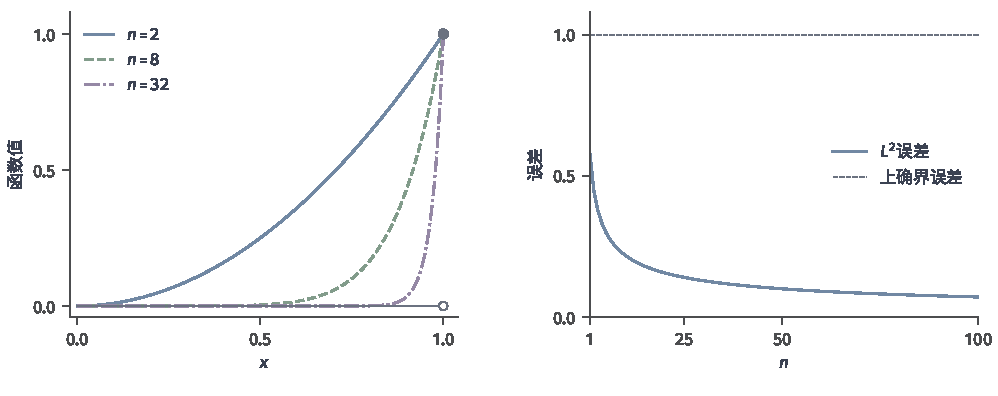
\includegraphics[width=169.0mm]{figures/01-mathematical-preliminaries-upper/01-mathematical-language-combinatorics-analysis-optimization/matplotlib/analysis-power-convergence-scales/figure.pdf}
  \caption{$x^n$在$[0,1]$上的两种整体尺度。左图蓝、绿、紫线分别取$n=2,8,32$；灰线与端点标记表示点态极限，
 它在$x<1$处为零、在$x=1$处为$1$。右图蓝色曲线为精确的$L^2$误差$(2n+1)^{-1/2}$，
 灰虚线为始终等于$1$的普通上确界误差；单点$x=1$的修改不影响积分。图为解析教学示例。}
 \label{fig:analysis-power-convergence-scales}
\end{figure*}

\paragraph{误差运算与极限存在}

把误差称为范数，还需要能控制误差相加。对$1<p<\infty$，令$q=p/(p-1)$，下面第一式要求$f\in L^p$、$g\in L^q$，第二式要求$f,g\in L^p$。Hölder不等式和Minkowski不等式分别给出
\begin{align}
 \int_X|fg|\,\mathrm d\mu&\leq\lVert f\rVert_p\lVert g\rVert_q,
 \label{eq:measurable-holder}\\
 \lVert f+g\rVert_p&\leq\lVert f\rVert_p+\lVert g\rVert_p.
 \label{eq:measurable-minkowski}
\end{align}
第一式控制乘积累计，第二式控制合并误差。对$p=1$，第二式直接来自逐点三角不等式；第一式的对应版本在$g$本质有界时为$\int|fg|\leq\lVert f\rVert_1\lVert g\rVert_{L^\infty}$，本质有界的定义在下一小小节给出。

Hölder可由非负实数$a,b$的标量不等式$ab\leq a^p/p+b^q/q$得到：当两个范数非零时，先把$f,g$除以各自范数，再对不等式积分，右侧为$1/p+1/q=1$。若某个范数为零，函数几乎处处为零，结论也成立。要得到Minkowski，先用$|f+g|^p\leq2^{p-1}(|f|^p+|g|^p)$确认和属于$L^p$，再写
\[
 \lVert f+g\rVert_p^p
 \leq\int_X(|f|+|g|)|f+g|^{p-1}\,\mathrm d\mu
 \leq(\lVert f\rVert_p+\lVert g\rVert_p)\lVert f+g\rVert_p^{p-1}.
\]
最后一步对两项分别用Hölder；若$\lVert f+g\rVert_p>0$，约去其$p-1$次幂即可。范围$p\geq1$有实际作用：在两点计数测度上，若$0<p<1$，$(1,0)$与$(0,1)$各有长度一，和的长度却是$2^{1/p}>2$，三角不等式失败。

误差还可以在不知道极限时判断：若$\lVert f_n-f_m\rVert_p\to0$于$n,m\to\infty$，就称它为$L^p$柯西列。对$1\leq p<\infty$，每个这样的函数列都有$L^p$极限，即$L^p$完备。下面说明极限如何构造。选子列$f_{n_k}$使$\lVert f_{n_{k+1}}-f_{n_k}\rVert_p\leq2^{-k}$，并令
\[
 H_M=|f_{n_1}|+\sum_{k=1}^M|f_{n_{k+1}}-f_{n_k}|.
\]
由Minkowski，$\lVert H_M\rVert_p\leq\lVert f_{n_1}\rVert_p+1$；令$H=\lim_M H_M$，非负单调收敛给出$\int_XH^p\,\mathrm d\mu\leq(\lVert f_{n_1}\rVert_p+1)^p<\infty$，因而$H$几乎处处有限。将$H$在可测零测集$\{H=\infty\}$上改为零后，就得到定义所要求的实值$L^p$代表。在修改前$H$有限的位置，相邻差绝对可加，所以$f_{n_k}$点态收敛到一个可测有限函数$f$；其余可测零测集上令$f=0$。同时$|f|\leq H$几乎处处，故$f\in L^p$。再用相邻差的尾和和单调收敛得到
\[
 \lVert f-f_{n_K}\rVert_p\leq\sum_{k=K}^{\infty}2^{-k}\longrightarrow0.
\]
原列的柯西条件与三角不等式便把子列收敛提升为整列的$L^p$收敛。这个构造保留的是积分误差意义下的极限；本章后面再研究这些空间上的结构和算子。

\subsubsection{忽略零测例外后的统一控制}
\paragraph{本质上确界与$L^\infty$误差}

普通上确界会被单个异常点改变，而保持可测性的零测集修改不影响积分。
若仍要控制最坏误差，却允许忽略测度为零的例外，就应比较函数绝对值的本质上界。
\begin{definition}[本质有界与绝对值的本质上界]
\label{def:analysis-essential-bound}
设$(X,\mathcal A,\mu)$为测度空间，$f:X\to\mathbb R$可测。其绝对值$|f|$的
\term{本质上确界}（essential supremum）定义为
\[   \operatorname*{ess\,sup}_{x\in X}|f(x)|   =   \inf\{M\geq0:|f(x)|\leq M\text{几乎处处}\}. \]
若集合中没有有限的$M$，上式取$+\infty$；若上式有限，就称$f$本质有界。
这里衡量的是$|f|$的大小，不是一般有符号函数$f$的本质上确界。
\end{definition}

将本质有界函数按几乎处处相同合并后，本质上界便给出等价类的长度：零长度恰好对应零等价类。
\begin{definition}[$L^\infty$空间与范数]
\label{def:analysis-linfty-space}
在同一测度空间上，$L^\infty(\mu)$由本质有界可测实函数的几乎处处等价类组成，
其范数定义为
\begin{equation}
  \lVert f\rVert_{L^\infty}
  =
  \operatorname*{ess\,sup}_{x\in X}|f(x)|.
\label{eq:analysis-essential-supremum-norm}
\end{equation}
同样用$f$代写等价类$[f]$；该范数不依赖代表元。
\end{definition}
例如在$[0,1]$上使用Lebesgue测度，令$f(0)=100$、其余位置$f(x)=0$，
则普通上确界为$100$，$|f|$的本质上确界却为$0$。
相应地，$\lVert f_n-f\rVert_{L^\infty}\to0$称为$L^\infty$收敛。
对每个$\varepsilon>0$，它要求某个$N$之后的全部误差都在几乎处处意义下
小于$\varepsilon$。可取精度$1/k$，把各$n,k$对应的可测零测例外并为一个零测集$E$；
于是存在同一个$E$，使$f_n$在$X\setminus E$上一致收敛。
反之，这种补集上的一致收敛立即给出$L^\infty$收敛。
因此它蕴含几乎处处收敛，却不一定是原集合上的一致收敛。
上面的$n\mathbb I_{\{0\}}$在$L^\infty$中恒等于零，普通上确界却为$n$。
对$x^n$，本质上确界误差仍为$1$，因为接近$1$的一整段正测度区间保留大误差，
不是删除端点就能消除。

$L^\infty$同样完备。若$f_n$为该范数下的柯西列，对每个精度$1/k$选出尾部范数界，并把可数个函数对及精度对应的可测零测例外取并。其补集上所有相应点值误差共同有界，因而$f_n$是一致柯西列；逐点取极限，例外集上置零，即得到本质有界的可测极限，并在$L^\infty$中收敛。这里沿用第~\ref{chap:univariate-calculus}章一致柯西的论证，只是先去掉了同一个零测集。

\paragraph{误差尺度的适用范围}

若$\mu(X)<\infty$且$f_n,f\in L^p$，一致收敛蕴含$L^p$收敛，因为
\[   \lVert f_n-f\rVert_p   \leq   \mu(X)^{1/p}\sup_{x\in X}|f_n(x)-f(x)|. \]
当空间测度无穷时，即使各项仍属于$L^p$，这个推论也可能失败。在$\mathbb R$上采用
Lebesgue测度，固定$1\leq p<\infty$，并取
\[
  f_n(x)=\frac1n\mathbb I_{[0,n^p]}(x).
\]
每个$f_n$都属于$L^p$，且$\sup_x|f_n(x)|=1/n\to0$，所以一致收敛到零；但
\[
  \lVert f_n\rVert_p^p=\frac{n^p}{n^p}=1,
\]
因而不在$L^p$中收敛到零。幅度虽降低，非零区域却同步扩大，累计误差没有随之减小。

反过来，积分误差小也不保证整列在几乎每个点收敛。
\begin{example}[小区间轮流扫过定义域]
\label{ex:analysis-lp-without-ae-limit}
在$[0,1)$上按轮次细分区间，令
\[
 f_{2^k+j}(x)=\mathbb I_{[j2^{-k},(j+1)2^{-k})}(x),
 \qquad k=0,1,\ldots,\quad j=0,\ldots,2^k-1.
\]
第$k$轮依次访问$2^k$个小区间，每个函数的$L^p$范数为$2^{-k/p}$，
所以对每个有限$p\geq1$，$f_n\to0$在$L^p$中成立。
但每个$x\in[0,1)$在每轮恰有一次取值$1$，也在无穷多个其他时刻取值$0$。
因此整列在每个$x$处都不收敛。积分看到每次被访问的区间越来越小，
点态收敛却要求同一个输入从某一时刻起一直稳定，这两个要求不能互代。
\end{example}

连续尖峰给出另一个比较。在式~\eqref{eq:measurable-continuous-spikes}中，
$b_n$处处趋零，且$\lVert b_n\rVert_p^p=1/[n(p+1)]\to0$，
但$\lVert b_n\rVert_{L^\infty}=1$。把峰高放大为$a_n=2nb_n$以后，
$\lVert a_n\rVert_1=1$，对$p>1$还有$\lVert a_n\rVert_p^p=2^pn^{p-1}/(p+1)$。
前面积分极限一节用这些尖峰说明逐点趋近不足以交换积分；这里则逐一计算它们在不同范数下的误差。

几乎处处和$L^p$范数还依赖所选测度：换一个测度，原先可忽略的集合可能重新变得重要。
若$Q$对$P$\term{绝对连续}（absolutely continuous），记作$Q\ll P$，则原来$P$
意义下的零测例外在$Q$下仍可忽略；
也就是对任意可测$A$，$P(A)=0$蕴含$Q(A)=0$。
这一测度关系保留的是零测集，不同于前面用距离控制输入、输出变化的映射连续性。
若没有$Q\ll P$，换分布可能给原零测集正质量。例如$P$是$[0,1]$上的均匀分布，
$Q$把全部质量放在$0$点；两个只在$0$处不同的函数在$P$意义下等价，在$Q$意义下
却可能具有完全不同的误差。
即使$Q\ll P$，$L^p$收敛也不能仅凭零测关系转移。令$P$是$(0,1)$上的长度测度，
$Q(A)=\int_A(2\sqrt x)^{-1}\,\mathrm dx$，其总质量为$1$，并有$Q\ll P$。
固定有限$p\geq1$，取$u_n=n^{1/(2p)}\mathbb I_{(0,1/n)}$，则
\[
 \lVert u_n\rVert_{L^p(P)}^p=n^{-1/2}\to0,\qquad
 \lVert u_n\rVert_{L^p(Q)}^p
 =\sqrt n\int_0^{1/n}\frac{\mathrm dx}{2\sqrt x}=1.
\]
$Q$虽没有给$P$零测集新增质量，却更看重靠近$0$的区域。
若另有统一常数$C$使$Q(A)\leq CP(A)$对所有可测$A$成立，
从简单函数经单调逼近可得$\lVert u\rVert_{L^p(Q)}
\leq C^{1/p}\lVert u\rVert_{L^p(P)}$，
此时才有直接的积分误差转移保证。
